% pruning-ww-case.tex

\documentclass{standalone}

\usepackage{tikz}
\usetikzlibrary{shapes, positioning, arrows.meta, decorations.pathmorphing}

\begin{document}
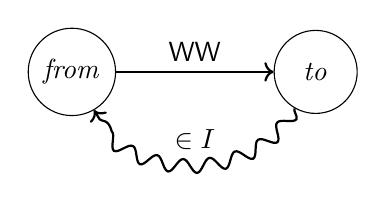
\begin{tikzpicture}[vertex/.style = {circle, draw, minimum size = 30pt},
  edge/.style = {->, thick},
  path/.style = {->, thick, decorate, decoration = snake}]

  \node[vertex] (from) {$\mathit{from}$};
  \node[vertex, right = 2.0cm of from] (to) {$\mathit{to}$};
  \draw[edge] (from) to node[above]{\textsf{WW}} (to);
  \draw[path] (to) to[bend left = 60] node[above]{$\in I$} (from);
\end{tikzpicture}
\end{document}